\subsection{Kontinuerlig afspilning}
\begin{frame}
	\frametitle{Kontinuerlig afspilning}
	\begin{itemize}
		\item Hvad skal vi gøre når der ikke er stemt på nogle sange
		\item Find en ny sang baseret på hvad der er blevet spillet
		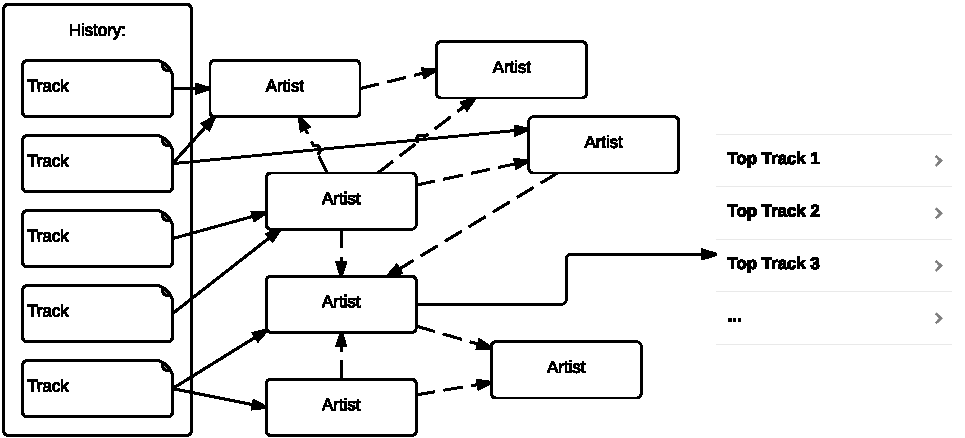
\includegraphics[width=270px]{slides/Frederik/algo}
	\end{itemize}
\end{frame}

\begin{frame}
\fontsize{8pt}{10}\selectfont
\frametitle{Kontinuerlig afspilning}
\begin{algorithmic}[1]
	\Function{findRelated}{$trackHistory$}
		\State{$tracksToLookAt = 9$}
		\State{$relatedArtists = empty list$}
		\If{$trackHistory.length < tracksTolookAt$}
			\State{$tracksToLookAt = trackHistory.length$}
		\EndIf{}
		\State{$lastPlayedTracks = trackHistory.getLast(tracksToLookAt)$}
		\ForAll{$track$ \textbf{in} $lastPlayedTracks$}
			\ForAll{$artist$ \textbf{in} $track.Artists$}
				\ForAll{$relatedArtist$ \textbf{in} $artist.relatedArtists$}
					\If{$relatedArtists.contains(relatedArtist)$}
						\State{$relatedArtist.count += 1$}
					\Else{}
						\State{$relatedArtists.add(relatedArtist)$}
						\State{$relatedArtist.count = 1$}
					\EndIf{}
				\EndFor{}
			\EndFor{}
		\EndFor{}
		\State{$mostRelated = null$}
		\ForAll{$artist$ \textbf{in} $relatedArtists$}
			\If{$mostRelated == null$ || $artist.count > mostRelated.count$}
				\State{$mostRelated = artist$}
			\EndIf{}
		\EndFor{}
		\ForAll{$track$ \textbf{in} $mostRelated.topTracks$}
			\If{$!lastPlayedTracks.contains(track)$}
			\State{}\Return{$track$}
			\EndIf{}
		\EndFor{}
	\EndFunction{}
\end{algorithmic}
\end{frame}


\begin{frame}
	\frametitle{Kontinuerlig afspilning}
	\begin{itemize}
		\item Algoritmen er aftestet uformelt
		\item Et eksempel på sange:
		\begin{itemize}
		\item Coldplay - A Sky Full of Stars
		\item Keane - Somewhere Only We Know
		\item Snow Patrol - Chasing Cars
		\item U2 - With or Without You
		\item The Killers - Mr. Brightside 
		\item Output: Muse - Madness
		\end{itemize}
	\end{itemize}
\end{frame}



\section{Refleksioner}
\subsection{Konklusion}

\begin{frame}
	\frametitle{Konklusion}
	\begin{itemize}
		\item How is it possible to develop a software solution which provides a venue with the ability to fairly and dynamically cater to their guests’ music preferences?
		\item How can the system provide supervision and control to the administrators?
		\item How can the system avoid undesirable music flow?
		\item Sikret at programmet lever op til krav, ved at være i tæt kontakt med brugere
	\end{itemize}
\end{frame}
\subsection{Afgrænsning}

\begin{frame}
	\frametitle{Afgrænsning}
	\begin{itemize}
		\item Offline afspilning
		\item Lockdown
		\item Sikkerhed
		\item Bruger autorisering
		\item Nem server opsætning og brug
	\end{itemize}
\end{frame}
\subsection{Fremtidig Udvikling}

\begin{frame}
	\frametitle{Fremtidig Udvikling}
	\begin{itemize}
		\item Fortsætte med iteration
		\item Rigtig context
	\end{itemize}
\end{frame}

{\aauwavesbg
\begin{frame}[plain,noframenumbering]
	\titlepage
\end{frame}}